\chapter{Introduction}
% uncomment the following line to create an unnumbered chapter
%\chapter*{Introduction}\addcontentsline{toc}{chapter}{Introduction}\markboth{Introduction}{Introduction}
%---------------------------------------------------------------
\setcounter{page}{1}

A few sentences about progressive line of cryptocurrencies and attacks related to them. Tell about security audits and how it is time consuming. Then a bit about LLM, which is developed in parallel. THen tel labout desire to interesct these 2 fields and describe sections of this thesis. 

\chapter*{Objectives}

Tell a bit about what was done and list objectives that were fullfilled:

\begin{itemize}
    \item Common vulnerability patterns and existing auditing methodologies of Ethereum smart contracts were studied.
    \item A state of the art review on the integration of Large Language Models for automated reasoning and the development of AI-based auditing agents was conducted.
    \item A system that integrates an LLM into the security auditing workflow was designed with further implementation, testing and evaluation.
    \item The obtained results, limitations, and potential improvements of LLM-based auditing systems were discussed in the end.
\end{itemize}


\chapter{Introduction}
% 1–2 pages. Problem, motivation, goal, contributions, and thesis roadmap.
\section{Motivation and Problem Statement}
% Why smart contract bugs are high impact (immutability, financial incentives) and why existing audits/tools still miss logical flaws.
\section{Research Objectives and Contributions}
% State your contribution precisely: extending Wake-AI with MCP-based RAG + building KB from Solidity vulns/audit knowledge.
\section{Thesis Structure}
% One paragraph explaining what each chapter delivers and how it connects.

\chapter{Ethereum}
This chapter introduces the foundations needed to understand Ethereum and the auditing methodologies developed in later chapters (TODO maybe change). It first explains generic \emph{blockchain} principles (as a technology family), then specializes to Ethereum’s execution model via the \emph{Ethereum Virtual Machine (EVM)} and the \emph{Solidity} language. The chapter closes with a concise taxonomy of common smart-contract vulnerabilities that will be referenced throughout the thesis.


\section{Overview}
Ethereum, formally launched in 2015, represents a significant evolution in blockchain technology. Originally proposed in a white paper by \textsc{Vitalik Buterin} in 2013/14, Ethereum extended the ledger-centric model into a full-fledged application layer offering smart contracts and decentralised applications (dApps) \cite{Buterin2013}. Rather than solely tracking value transfers, Ethereum enables arbitrary programmable logic through the EVM execution environment, while preserving the core blockchain properties of transparency, decentralisation and immutability \cite{wood2014yellow}. By doing so, it transformed the blockchain into a generalised state-transition machine, thereby broadening its applicability far beyond simple currency use-cases.


\subsection{Blockchain}
% Blocks/transactions/state; keep it tight and oriented toward contract execution.
\subsection{Accounts and Transactions}
% EOAs vs contract accounts; call semantics at high level (sets up msg.sender, msg.value, calldata).
\subsection{Consensus mechanisms}
In a PoW system, network participants (miners) compete to solve computational puzzles (e.g., find a nonce so that the hash of the block header meets a target) and thereby propose the next valid block. :contentReference[oaicite:8]{index=8} In contrast, PoS selects block proposers (validators) based on their stake in the network (i.e., the amount of tokens locked up) rather than raw computing power, thereby altering the incentive, security and energy-profile of the system. :contentReference[oaicite:9]{index=9}

\subsubsection*{Proof of Work}
Proof-of-work (PoW) is an algorithm that sets the difficulty level and rules governing the activities of miners on PoW-based blockchains. Mining represents
the ’work’ needed to validate and append legitimate blocks to the blockchain.
This process is crucial as it directly affects the blockchain’s length, thereby
helping the network determine the most accurate progression of the chain.
As miners continue to solve complex mathematical problems, thereby adding
more blocks, the blockchain grows longer, which improves the network’s confidence in the current state of the ledger. This chain lengthening also increases
security by making altering any information in previous blocks increasingly
difficult. This consensus mechanism is used in the most popular blockchain
implementation, called Bitcoin.

\subsubsection*{Proof of Stake}
Proof of Stake (PoS) is an essential consensus algorithm that defines the rules
and mechanisms for participants in PoS-based blockchains. In PoS, the process of ’staking’—rather than mining—serves as the mechanism through which
validators are chosen to confirm transactions and create new blocks. Validators are selected based on the amount of cryptocurrency they hold and are
willing to ’stake’ as collateral. This process is critical as it helps ensure the
security and accuracy of the blockchain by encouraging validators to act honestly to avoid losing their stakes. As more blocks are validated and added to
the chain, the blockchain becomes longer and more robust, thereby upgrading
the network’s trust in the current ledger. This method increases the efficiency
of the validation process and reduces the energy consumption compared to
proof-of-work systems, making it a more environmentally friendly alternative.
The most used blockchain that uses the proof-of-stake mechanism is Ethereum

\section{Ethereum Virtual Machine}
The Ethereum Virtual Machine (EVM) is a deterministic state machine that executes the bytecode of the smart contract identically on all nodes \cite{wood2014yellow}. However, it is not Turing complete in the classical sense: execution is strictly resource-bounded by gas - every instruction has a metered gas cost, and execution halts once the supplied gas is exhausted. 
This gas-bounded execution guarantees termination and prevents non-halting or deliberately expensive programs from stalling the network; accordingly, the EVM is often described as \emph{quasi–Turing complete} (computationally universal only under a finite gas budget) \cite{antonopoulos2018mastering}\cite{wood2014yellow}.

\subsection{Gas}
Gas is the unit of account for computational effort in Ethereum. Each EVM opcode has an associated gas cost, and a transaction specifies an upper bound (gas limit) on how much gas may be consumed during its execution.

Gas serves three core purposes: 
\begin{itemize}
    \item \emph{metering} computation and storage, so that the use of the resources is paid for by the initiator of a transaction.
    \item \emph{DoS resistance} and spam prevention, because excessively resource-intensive executions become economically infeasible \cite{wood2014yellow}\cite{article_1559}.
    \item \emph{economic prioritization} of limited block space via fees
\end{itemize}

Since EIP-1559\footnote{\url{https://eips.ethereum.org/EIPS/eip-1559}}, each block includes a dynamically adjusted \emph{base fee} that is burned and a user-specified \emph{priority fee} (tip) paid to the block proposer. 
Users submit \texttt{maxFeePerGas} and \texttt{maxPriorityFeePerGas}; the effective price paid per gas equals \(\min(\texttt{maxFeePerGas}, \text{base fee} + \texttt{maxPriorityFeePerGas})\). 
Blocks have an elastic gas target and the base fee increases or decreases depending on recent block gas usage, stabilizing the fee market while preserving incentives.


\subsection{Architecture}

\begin{figure}[!htbp]
    \centering
    \includegraphics[width=\linewidth]{images/evm}
    \caption{Ethereum Virtual Machine illustration TODO REF.}
    \label{fig:evm}
\end{figure}

where 
\begin{itemize}
    \item Program Counter (PC) - component that tracks the current instruction that it is executing;
    \item EVM code - immutable compoennt holds the bytecode of the smart contract that is being executed.
    \item Account Storage - part of the persistent state of the blockchain where the data of smart contracts are stored permanently. There are two types of accounts in the Ethereum environment:\texttt{ (i) }Externally Owned Account (EOA) that is owned by any external entity. Most commonly, it is referred to as a user account; and\texttt{ (ii) }Smart Contract Account that is owned by a smart contract and often controlled by an EOA that interacts with the deployed smart contract \cite{Buterin2013}.
\end{itemize}

\subsection{Memory}

\begin{itemize}
    \item \textbf{Stack} - low-level memory structure that operates on a last-in, first-out (LIFO) principle. It stores small local variables and value types that are required for immediate execution. The stack is limited to 1024 elements, each 256 bits wide, and is accessible only through EVM opcodes or inline assembly. Careful management is essential, as exceeding its capacity causes the execution of the contract to fail \cite{evm_storage}.
    \item \textbf{Memory} - dynamic and expandable storage area allocated for each function execution, which is then discarded once the function has finished. Unlike the stack, which is restricted to temporary data storage, memory allows for more flexible and longer-lived data retention.
    \item \textbf{Storage} - persistent storage is associated with every smart contract and holds its state. Read and write operations in storage are relatively more expensive than those performed in memory. The data in storage are maintained as key-value pairs \cite{evm_storage_arxiv}.
    \item \textbf{Calldata} - read-only and immutable storage that holds function arguments and transaction data for the duration of a transaction call.
\end{itemize}

\section{Smart Contracts}
% Solidity only to the extent necessary for your later vulnerability patterns + tool parsing.
\subsection{Solidity}


\section{Security}
% Introduce security mindset: assets, adversary model, invariants, threat boundaries.
\subsection{Vulnerability Taxonomies}
% Use OWASP SC Top 10 + SWC as your naming backbone (consistent labels throughout thesis).
% Cite OWASP + SWC. :contentReference[oaicite:12]{index=12}
\subsection{Vulnerability Patterns (Practical)}
% Your “working set” of patterns referenced later by the KB.
\subsubsection*{Reentrancy and External Call Hazards}
\subsubsection*{Access Control and Authorization Bugs}
\subsubsection*{Arithmetic / Precision / Accounting Errors}
\subsubsection*{DoS and Gas Griefing}
\subsubsection*{Front-running / MEV-related Issues (when relevant)}
\subsubsection*{Upgradeability and Initialization Bugs}
% For each: 2–5 sentences + 1 tiny example later in Implementation/Eval if needed.

\section{Audit Methodology}

Smart contract auditing has evolved into a specialized discipline that combines elements of traditional software security review with domain-specific knowledge about blockchain systems and economic attack vectors. Unlike conventional software where bugs might cause crashes or data corruption, smart contract vulnerabilities can lead directly to financial losses, often measured in millions of dollars TODO(\cite{some_link/footnote}).

Auditors begin by establishing what the system is supposed to do and identifying potential threat vectors, then systematically examine the implementation through a combination of manual review and automated tools. While human expertise remains central to catching subtle logic bugs and business logic flaws, automation has become increasingly important for handling the scale and complexity of modern DeFi protocols \cite{perez2021smart}. 

\subsubsection*{System overview}

\subsubsection*{Trust model}

Before examining a single line of code, effective audits begin with understanding what the system is designed to do and what could go wrong. This specification and threat modeling phase establishes the foundation for all subsequent analysis. Auditors work with the development team to document the intended behavior of the protocol, including state invariants that should always hold, access control assumptions about who can perform which actions, and economic mechanisms that should remain balanced under all circumstances \cite{groce2018echidna}.

State invariants are particularly critical in DeFi protocols. For example, an automated market maker (AMM) might have an invariant that the product of token reserves remains constant except during fee accrual, or a lending protocol might require that total collateral always exceeds total debt by some minimum margin. Documenting these invariants explicitly serves multiple purposes: it guides manual review by clarifying what properties to verify, it provides targets for property-based fuzzing tools, and it establishes success criteria for testing. When invariants are violated, it often indicates either a vulnerability in the code or a gap in the original specification that needs addressing.

Trust assumptions define the threat model—which actors are assumed to be honest, which might be malicious, and what capabilities each has. A typical DeFi protocol might trust its governance multi-sig to upgrade contracts responsibly while assuming that all regular users will act to maximize their own economic benefit, including front-running transactions and exploiting any profitable vulnerabilities. External dependencies also factor into the trust model: does the protocol rely on specific oracle providers, and what happens if those oracles are compromised or manipulated? These assumptions directly influence what the auditor looks for in the code.

This phase also identifies high-value targets—the functions and state variables most critical to protocol security and most likely to be attacked. In a lending protocol, this might be functions that calculate collateralization ratios or trigger liquidations. In a bridge, it could be the validation logic for cross-chain messages. By explicitly mapping out these critical components and their security requirements up front, auditors can allocate their limited time more effectively and ensure comprehensive coverage of the attack surface. This specification work also sets up what an LLM-based agent should retrieve when analyzing code: knowing the declared invariants and trust assumptions allows the agent to focus its limited context window on retrieving code segments most relevant to verifying those properties.

\subsubsection{Manual Code Review}

Manual code review remains the cornerstone of smart contract auditing despite advances in automation. Experienced auditors develop intuition about common vulnerability patterns, but more importantly, they can reason about complex interactions, business logic edge cases, and economic attack vectors that current tools struggle to identify. The review process typically proceeds through several phases, each with a different focus and level of detail.

The review begins with architectural analysis—understanding how contracts interact, what external systems they depend on, and how data flows through the protocol. Auditors construct mental models (and often diagrams) of the system's components and their relationships. For example, in a yield aggregation protocol, they map out how user deposits flow into various strategies, how yield is calculated and distributed, and what happens during rebalancing or emergency withdrawals. This high-level understanding helps identify architectural vulnerabilities like dangerous centralization points, circular dependencies that could create reentrancy opportunities, or reliance on external systems that could fail.

With the architecture clear, auditors move to examining critical execution paths. They trace through key user interactions step by step: what happens when Alice deposits tokens, when Bob triggers a liquidation, when governance proposes a parameter change? This path analysis helps identify missing checks, incorrect sequencing, or edge cases where the code behaves unexpectedly. Auditors pay special attention to paths involving external calls, token transfers, and state changes—the operations most likely to introduce vulnerabilities.

Invariant verification forms another crucial part of manual review. Armed with the invariants documented during threat modeling, auditors examine whether the code actually maintains these properties under all possible executions. This often involves reasoning about potential sequences of function calls and state transitions. For instance, if a protocol claims that "users can always withdraw their proportional share of pooled assets," the auditor checks whether there are any code paths where this could fail—perhaps during contract upgrades, when certain functions are paused, or in response to specific market conditions.

Edge case analysis requires creativity and experience. Auditors consider boundary conditions: what happens with zero values, maximum values, or just-below-overflow values? They think about timing issues: what if a transaction is front-run, what if the block timestamp is manipulated slightly, what if multiple operations happen in the same block? They examine error handling: are all failure modes properly addressed, or are there paths where errors could leave the system in an inconsistent state? This type of reasoning is difficult to automate because it requires understanding both the code's literal behavior and the protocol's semantic intent.

The manual review process is inherently limited by human cognitive constraints. An auditor can only hold so much context in working memory at once, and complex protocols might span dozens of contracts with thousands of lines of code. This is where tool-assisted workflows become valuable—not to replace human judgment, but to help auditors manage complexity by automating context retrieval, flagging potential issues for human investigation, and maintaining consistency in coverage across a large codebase. The goal of integrating LLMs into this workflow is to augment human auditors with better information retrieval and pattern recognition, allowing them to focus their expertise on the creative reasoning tasks that machines still cannot perform.

\subsubsection*{Static analysis}

\subsubsection*{Local deployment}

\subsubsection*{Tool-Based Analysis}

Automated analysis tools have become an essential part of the smart contract audit workflow, complementing manual review by efficiently checking for known vulnerability patterns and coding errors. These tools vary in their approaches—from lightweight pattern matching to sophisticated symbolic execution—and each brings different strengths and limitations to the audit process.

Static analysis tools examine code without executing it, using techniques ranging from simple syntactic pattern matching to complex abstract interpretation. Slither, developed by Trail of Bits, has emerged as one of the most widely adopted static analyzers for Solidity \cite{feist2019slither}. It operates on Solidity's intermediate representation (IR) and includes over 70 built-in detectors for common issues like reentrancy vulnerabilities, unprotected ether withdrawals, incorrect ERC-20 implementations, and dangerous delegatecalls. Slither's strength lies in its speed and comprehensive coverage—it can analyze a medium-sized project in seconds and rarely produces false negatives for the patterns it targets.

However, static analyzers face fundamental limitations. They must over-approximate program behavior to be sound, which often leads to false positives—flagging code as potentially vulnerable when it's actually safe. For example, Slither might flag a reentrancy warning for any external call followed by a state change, even when the specific call cannot actually re-enter the contract. Auditors must manually review these warnings to separate real issues from noise. More critically, pattern-based detectors can only find vulnerabilities they were explicitly programmed to recognize. Novel vulnerability classes or complex logic bugs that don't match known patterns slip through entirely.

Other static analysis tools take different approaches. Mythril employs symbolic execution and SMT solving to explore possible execution paths and find states that violate security properties \cite{mueller2018mythril}. This can uncover deeper issues than pattern matching, but symbolic execution doesn't scale well to large contracts or complex path conditions—the number of possible paths grows exponentially with program size and branching. Securify uses a dataflow analysis framework and security patterns specified in a domain-specific language \cite{tsankov2018securify}, offering more flexibility in specifying what to look for but requiring expertise to write effective patterns.

Linters like Solhint and Ethlint catch style violations and potential code quality issues rather than security vulnerabilities per se. While less critical than security-focused analyzers, they help maintain code quality that makes contracts easier to audit. They flag issues like missing visibility specifiers, unused variables, overly complex functions, and deviations from best practice patterns like checks-effects-interactions.

Integration of multiple tools provides better coverage than relying on any single analyzer. A typical audit workflow might run Slither for quick pattern detection, Mythril for deeper analysis of critical functions, and various linters for code quality checks. However, this multi-tool approach creates new challenges: each tool has its own output format, overlapping detections need deduplication, and the auditor must triage dozens or hundreds of findings to identify which require attention.

This is where the Wake framework becomes relevant to our work. Wake provides a Python-based infrastructure for building custom detectors and integrating various analysis tools in a unified workflow \cite{wake2023documentation}. Unlike standalone tools that operate in isolation, Wake allows auditors to write detectors that combine insights from multiple sources—for example, using both AST pattern matching and data flow analysis to reduce false positives. Wake's Python ecosystem also makes it a natural bridge to LLM-based analysis: we can extract rich context from Wake's analysis passes and feed it to language models that can reason about patterns too complex for rule-based systems.

The key insight for our work is that automated tools excel at scalable, repeatable pattern matching but struggle with novel vulnerabilities and contextual reasoning. Meanwhile, LLMs demonstrate strong pattern recognition on code they've seen during training and can generate natural language explanations, but they lack the precision and soundness guarantees of formal methods. By combining static analysis tools with LLM reasoning in an agent-based architecture—using tools like Wake to extract structured information and RAG to provide relevant context—we aim to get closer to the best of both approaches.

\subsubsection*{Local deployment}

Testing smart contracts in realistic conditions requires deploying them to a local blockchain environment where their behavior can be observed without risking real funds or incurring transaction costs. Modern development frameworks like Hardhat, Foundry, and Wake provide robust local testing infrastructure that has become standard in the audit workflow \cite{hardhat2023, foundry2023}.

Unit tests verify individual functions in isolation, checking that they produce expected outputs for given inputs and properly handle error conditions. Integration tests examine how multiple contracts interact, ensuring that complex workflows execute correctly end-to-end. For example, testing a lending protocol might involve simulating a sequence of deposits, borrows, interest accrual, and liquidations to verify that all state transitions occur correctly and invariants are maintained. Well-written test suites serve both as verification of correct behavior and as documentation of intended functionality.

Fork testing represents a particularly powerful technique for smart contract auditing. Rather than testing in isolation, fork testing deploys the contract under audit to a local blockchain that has copied the state of mainnet at a specific block. This allows the contract to interact with real deployed protocols—actual DEXes, oracles, tokens—without requiring the auditor to mock these complex systems. For example, when auditing a yield optimization strategy, fork testing can verify that the strategy actually generates yield when deployed against real DeFi protocols, that it handles real market conditions correctly, and that it responds appropriately to real oracle updates.

Fork testing also enables reproduction and investigation of historical exploits. By forking at a block just before a known attack, auditors can replay the attack transaction to understand exactly how it worked, then test whether proposed fixes would have prevented it. This forensic capability helps validate that audit recommendations actually address the vulnerabilities they target. Wake's testing framework includes sophisticated fork testing capabilities, allowing tests to manipulate fork state, impersonate arbitrary accounts, and observe detailed execution traces.

Despite their value, tests have inherent limitations. Test coverage is only as good as the test cases written—they can demonstrate the presence of bugs but never prove their absence. Auditors who rely too heavily on "the tests pass" as evidence of security may miss edge cases that weren't considered when writing tests. Additionally, tests typically focus on expected usage patterns, while attackers deliberately seek unexpected input combinations and state transitions that developers didn't anticipate.

This limitation motivates property-based testing approaches, where instead of writing individual test cases, auditors specify properties that should always hold and let the testing framework automatically generate inputs trying to violate those properties. This bridges to our next topic: fuzz testing, which takes this idea even further by using randomization and evolutionary algorithms to explore the state space more thoroughly than human-written tests ever could.

\subsubsection*{Fuzz testing}

Fuzzing has emerged as one of the most effective techniques for uncovering subtle bugs in smart contracts, particularly logic errors that evade static analysis and aren't covered by manual test cases. Unlike traditional testing where humans specify input values, fuzzing automatically generates large numbers of random or semi-random inputs to explore program behavior across a wide range of scenarios \cite{trail2023fuzz}.

The simplest form of fuzzing, random input generation, feeds functions with arbitrary values and checks whether they crash, revert unexpectedly, or violate assertions. While naive, this approach can quickly find boundary condition bugs—what happens with zero values, maximum uint256 values, or unexpected combinations? More sophisticated fuzzers use coverage-guided generation, tracking which code paths have been executed and favoring inputs that reach new branches. This evolutionary approach efficiently explores the state space, focusing computational effort on finding inputs that trigger novel behaviors.

Property-based fuzzing, exemplified by tools like Echidna \cite{grieco2020echidna} and Foundry's fuzzer \cite{foundry2023}, takes this further by allowing auditors to specify invariants that should always hold. The fuzzer then attempts to find any sequence of function calls and inputs that violates these invariants. For example, an auditor might specify that "total shares times share price should equal total assets" for a vault contract. The fuzzer will generate thousands of random deposit, withdraw, and transfer operations, checking after each whether this invariant still holds. When it finds a violation, it automatically minimizes the test case to the simplest sequence that reproduces the issue.

Stateful fuzzing considers sequences of operations rather than isolated function calls. Many vulnerabilities only emerge through specific state transitions—for example, a reentrancy bug that requires calling function A to set up state, then reentering during a call to function B to exploit that state. Echidna maintains a model of contract state and generates sequences of transactions that explore different state transition paths. This catches bugs that unit tests miss because the test writer didn't consider that particular sequence of operations.

Fuzzing excels at finding logic bugs—violations of business rules or implicit assumptions that static analyzers can't detect because they aren't simple pattern matches. For instance, fuzzing might discover that a specific sequence of deposits and withdrawals allows a user to extract more funds than they deposited, or that under certain market conditions a pricing oracle can be manipulated. These are precisely the high-impact bugs that make auditing challenging: they're correct in terms of type safety and basic invariants, but incorrect in terms of the protocol's economic logic.

However, fuzzing has limitations. It's probabilistic rather than exhaustive—finding a bug depends on the fuzzer happening to generate the right sequence of inputs, which might be a tiny fraction of the total input space. Complex bugs requiring specific state setups might be missed if the fuzzer doesn't happen to explore that path. Additionally, writing good invariant specifications requires expertise—if the auditor doesn't correctly specify what should always be true, the fuzzer won't detect violations.

The integration of fuzzing into the audit workflow has become standard practice. Auditors typically run fuzzers overnight or over weekends, generating millions of test cases to explore state spaces too large for manual testing. When combined with static analysis (which finds known patterns quickly) and manual review (which applies human reasoning about business logic), fuzzing provides a powerful third pillar in the defense against vulnerabilities. For our work with LLM-based agents, fuzzing results provide valuable signal: when a fuzzer finds an invariant violation, the LLM can analyze the failing sequence to explain why it violates the invariant and suggest fixes.

Rather than viewing automation as competing with human auditors, we see it as extending their capabilities. The techniques we've discussed generate vast amounts of information: static analyzers flag hundreds of potential issues, tests exercise thousands of state transitions, fuzzers generate millions of inputs. Making effective use of this information requires systems that can retrieve relevant context, synthesize insights across tools, and present findings in ways that augment human reasoning.

The code analysis approaches we examine next build on the audit methodology foundations established here. We explore how static analysis frameworks like Wake provide structured access to code properties, how retrieval systems can surface relevant code segments for LLM analysis, and how agent architectures can orchestrate multiple tools to tackle complex analysis tasks. The goal is not to replace the auditor workflows described in this chapter, but to make them more efficient and effective by automating the retrieval and synthesis steps that currently consume significant auditor time.

\chapter{Code analysis}
% Goal: describe analysis methods you’ll reference when positioning Wake/Wake-AI and your RAG design.
\section{Static analysis}
% “Analysis without execution”: representations + algorithms.
\subsection{Abstract syntax tree}
% Structure, why good for pattern matching and feature extraction.
\subsection{Intermediate representation}
% Why IR helps normalize Solidity constructs; connect to Wake’s internal model later.
\subsection{Control flow analysis}
% Paths, reachability, call graph; key for reentrancy/authorization flows.
\subsection{Data flow analysis}
% Def-use, taint sources/sinks; explain limitations with aliasing/solidity specifics.
\subsection{Inter-procedural analysis}
% Cross-function reasoning, summaries, scalability tradeoffs.

\section{Dynamic analysis}
% “During execution”: what you can observe that static misses.
\subsection{TODO}
% Transaction traces, revert reasons, state diffs (keep conceptual).
\subsection{Fuzz testing}
% Stateful fuzzing, invariants, corpus guidance; connect to Wake fuzzing later.

\section{Formal verification}
% Position it as strongest guarantees but costly; relevant as future work / complementary checks.
\subsection{Symbolic execution}
% Path explosion, environment modeling; mention common tools as examples (no long tool survey).
\subsection{Model checking}
% Properties/invariants, finite abstraction.
\subsection{Theorem proving}
% Very brief, mainly to contextualize “verification” as a baseline you don’t fully implement.
\section{Summary and Transition to LLM-based Analysis}

\chapter{Large Language Models}

The detection of vulnerabilities in smart contracts has traditionally relied on rule-based static analysis tools and formal verification methods. While these approaches have proven effective for certain classes of vulnerabilities, they struggle with complex logic bugs and require extensive manual effort to develop detection rules \cite{luu2016making, tsankov2018securify}. Recent advances in deep learning, particularly the emergence of transformer-based Large Language Models (LLMs), have opened new possibilities for automated vulnerability detection that can learn patterns from code rather than relying solely on pre-defined rules \cite{chen2021evaluating, wang2024software}.

This chapter explores the architectural foundations of modern LLMs and their application to vulnerability detection in smart contracts. We begin by tracing the evolution from early neural network approaches to the transformer architecture that underlies contemporary LLMs. Understanding these foundations is essential for our later discussion of how Wake-AI leverages LLM capabilities and why techniques like Retrieval-Augmented Generation (RAG) and Model Context Protocol (MCP) become necessary when working with the constraints of real-world code analysis tasks.

\section{Transformers}

\begin{figure}[!htbp]
    \centering
    \includegraphics[width=0.7\linewidth]{images/transformer.png}
    \caption{Transformer TODO REF.}
    \label{fig:transformer}
\end{figure}

Before diving into transformer architecture, it's worth briefly reviewing the path that led to their development. Early attempts to apply machine learning to code analysis relied on simpler models such as n-gram language models and basic recurrent neural networks \cite{hindle2012naturalness}. These approaches treated code as a sequence of tokens and attempted to learn statistical patterns that could distinguish vulnerable from secure code.

Recurrent Neural Networks (RNNs) and their more sophisticated variants, Long Short-Term Memory (LSTM) networks \cite{hochreiter1997long}, represented a significant step forward. By maintaining hidden states that captured information about previously seen tokens, LSTMs could theoretically model long-range dependencies in code. However, they suffered from fundamental limitations. The sequential nature of RNN processing meant that information had to be passed through many intermediate states to connect distant parts of a program, leading to the vanishing gradient problem during training \cite{bengio1994learning}. More critically, the sequential processing constraint prevented parallelization, making it impractical to train on the massive code corpora needed for general-purpose code understanding.

The transformer architecture, introduced by Vaswani et al. in their seminal 2017 paper "Attention Is All You Need" \cite{vaswani2017attention}, fundamentally changed this landscape. By replacing sequential recurrence with attention mechanisms that could directly relate any two positions in a sequence, transformers eliminated the sequential bottleneck while providing more direct paths for gradient flow during training. This architectural shift enabled both the massive scale of modern LLMs and their superior ability to capture complex relationships in code.

\section{Transformer Architecture}

The transformer architecture consists of an encoder-decoder structure, though many modern LLMs use only the decoder portion (GPT-family models) or only the encoder portion (BERT-family models) \cite{radford2019language, devlin2019bert}. Figure~\ref{fig:transformer} illustrates the complete transformer architecture. For vulnerability detection tasks, we primarily work with decoder-only models that have been pre-trained on large code corpora and can generate natural language explanations of detected issues.

At its core, a transformer processes sequences through a series of identical layers, each containing two main components: a multi-head self-attention mechanism and a position-wise feed-forward network. The architecture also employs residual connections around each of these sub-layers, followed by layer normalization \cite{ba2016layer}.

The input to the transformer begins with token embeddings that represent each element of the input sequence as a dense vector. For code analysis, these tokens might represent keywords, identifiers, operators, and other syntactic elements of the programming language. Crucially, since the attention mechanism itself has no inherent notion of sequence order, positional encodings are added to these embeddings to inject information about token positions.

\subsection{Self-Attention Mechanism}

The self-attention mechanism is the defining innovation of transformer architecture. Unlike RNNs that process tokens sequentially, self-attention allows the model to directly compute relationships between all pairs of tokens in parallel. This capability is particularly valuable for code analysis, where understanding a vulnerability often requires relating elements that are far apart in the token sequence—for example, connecting a variable declaration to its use in a security-critical operation several functions away.

The attention mechanism operates through three learned linear projections of the input: queries (Q), keys (K), and values (V). For each position in the sequence, the model computes attention scores that determine how much focus to place on every other position. Mathematically, the attention operation for a single head is defined as:

\begin{equation}
\text{Attention}(Q, K, V) = \text{softmax}\left(\frac{QK^T}{\sqrt{d_k}}\right)V
\end{equation}

where $d_k$ is the dimension of the key vectors \cite{vaswani2017attention}. The scaling factor $\sqrt{d_k}$ prevents the dot products from growing too large in magnitude, which would push the softmax function into regions with extremely small gradients.

To understand this intuitively, consider analyzing a function call in Solidity code. The query represents "what am I looking for" from the perspective of each token. The keys represent "what information do I contain" from each token's perspective. The dot product $QK^T$ computes compatibility scores between queries and keys—essentially asking "how relevant is each token to each other token?" The softmax normalizes these scores into a probability distribution, and finally, this distribution is used to take a weighted average of the values, producing an attention-weighted representation.

Multi-head attention extends this by running several attention operations in parallel, each with different learned projection matrices. The outputs are concatenated and linearly transformed:

\begin{equation}
\text{MultiHead}(Q, K, V) = \text{Concat}(\text{head}_1, ..., \text{head}_h)W^O
\end{equation}

where each $\text{head}_i = \text{Attention}(QW^Q_i, KW^K_i, VW^V_i)$ \cite{vaswani2017attention}. This multi-head design allows the model to attend to information from different representation subspaces simultaneously. In practice, different attention heads often learn to capture different types of relationships—some might focus on syntactic structure, while others capture semantic relationships or data flow patterns \cite{clark2019does, vig2019analyzing}.

For vulnerability detection, this multi-head attention proves particularly powerful. One attention head might learn to track variable definitions and uses, another might focus on function call chains, and yet another might specialize in recognizing common vulnerability patterns. The model can then combine these different perspectives to make more nuanced judgments about potential security issues.

The transformer architecture includes two variants of attention: in the encoder, self-attention allows each token to attend to all tokens in the input sequence. In the decoder, masked self-attention restricts each token to only attend to previous tokens (and itself), which is essential for autoregressive generation tasks. When we use a pre-trained LLM for vulnerability analysis, we're typically leveraging this masked attention structure—the model has learned to predict subsequent tokens given previous context, and this predictive capability extends to understanding what code patterns might indicate vulnerabilities.

\subsection{Positional Encoding and Context Windows}

A fundamental characteristic of the attention mechanism is its permutation invariance: if we shuffled the input tokens, the attention computation would produce the same results (just in shuffled order). For natural language and code, where token order carries critical semantic information, this is clearly problematic. Positional encoding solves this by adding position-dependent signals to the token embeddings before they enter the transformer layers.

The original transformer used sinusoidal positional encodings \cite{vaswani2017attention}:

\begin{equation}
PE_{(pos, 2i)} = \sin\left(\frac{pos}{10000^{2i/d_{model}}}\right)
\end{equation}
\begin{equation}
PE_{(pos, 2i+1)} = \cos\left(\frac{pos}{10000^{2i/d_{model}}}\right)
\end{equation}

where $pos$ is the position in the sequence, $i$ is the dimension index, and $d_{model}$ is the model dimension. This encoding has useful mathematical properties: any fixed offset in position corresponds to a linear transformation in the encoding space, potentially allowing the model to learn to attend by relative positions. Moreover, these functions can extend to sequence lengths beyond those seen during training.

However, many modern LLMs use learned positional embeddings instead \cite{devlin2019bert, radford2019language}. While these must be explicitly trained for each position up to a maximum sequence length, they offer more flexibility and often perform slightly better in practice. More recent approaches like Rotary Position Embedding (RoPE) \cite{su2021roformer} and ALiBi \cite{press2022train} have shown promise in extending effective context lengths beyond training limits, an important consideration for analyzing long smart contracts.

The concept of a \textit{context window} refers to the maximum number of tokens a model can process at once. This is a hard constraint imposed by both the positional encoding scheme and computational resources—attention has $O(n^2)$ complexity with sequence length $n$, making it expensive for very long sequences. Early transformer models worked with context windows of 512 or 1024 tokens \cite{vaswani2017attention, devlin2019bert}. Modern LLMs have dramatically expanded this: GPT-4 supports context windows up to 128,000 tokens \cite{openai2023gpt4}, and Claude 3 extends to 200,000 tokens \cite{anthropic2024claude}.

For smart contract analysis, context window limitations pose a significant practical challenge. A typical smart contract might contain 500-2000 lines of Solidity code, which can translate to 5,000-20,000 tokens once we include relevant context like imported libraries, interface definitions, and documentation. More complex projects might exceed even generous context limits. This constraint motivates the need for Retrieval-Augmented Generation (RAG) approaches, which we explore in the next chapter. Rather than feeding an entire codebase into the model at once, RAG systems selectively retrieve the most relevant code segments, allowing the LLM to focus its limited context window on the information most likely to contain or explain vulnerabilities.

The feed-forward networks in each transformer layer also play a crucial role, though they're often overshadowed by the attention mechanism in discussions. After attention aggregates information across the sequence, the feed-forward network applies the same learned transformation to each position independently:

\begin{equation}
\text{FFN}(x) = \max(0, xW_1 + b_1)W_2 + b_2
\end{equation}

This two-layer network with ReLU activation significantly expands the model's capacity to learn complex patterns \cite{vaswani2017attention}. Recent work suggests these feed-forward layers serve as "key-value memories" where the model stores factual knowledge learned during pre-training \cite{geva2021transformer}.

Understanding these architectural components is essential for effectively applying LLMs to vulnerability detection. The attention mechanism's ability to capture long-range dependencies helps identify vulnerabilities that involve interactions between distant parts of code. The multi-head design allows specialization for different types of patterns. And the context window constraints explain why we need sophisticated retrieval strategies to handle real-world smart contracts. In the following chapters, we examine how these capabilities and limitations shape our approach to building Wake-AI, a system that combines static analysis tools like Wake with the pattern-recognition abilities of modern LLMs.


\section{Training paradigms}
\subsection{Pre-training}
\subsection{Fine-tuning}
\subsection{Prompting}

\section{Code-Specialized Models and Embeddings}
% Explain why code models/embeddings help retrieval + similarity search (ties directly to your KB).
\subsection{Encoder Models for Code (e.g., CodeBERT)}
\subsection{Seq2seq Code Models (T5/CodeT5 family)}
\subsection{Code Embeddings for Retrieval}
% Put nomic-embed-code here if you used it; otherwise keep model-agnostic and mention you pick one in Implementation.

\section{State of the Art: LLMs in Smart Contract Auditing}
% Focus on 4 buckets: prompt-only, agentic, fine-tuned, RAG-augmented.
\subsection{Prompt-Only and Agentic Auditing Pipelines}
% Example: multi-agent approaches; cite one solid paper you actually discuss.
\subsection{Fine-tuned Models for Smart Contract Vulnerability Detection}
% Example: SmartLLM (RAG + fine-tuning). :contentReference[oaicite:15]{index=15}
\subsection{RAG-Augmented Detection Frameworks}
% Discuss ParaVul (explicit RAG + verification/fusion). :contentReference[oaicite:16]{index=16}
% (This directly motivates your “RAG inside Wake-AI” choice.)

\section{Prompting strategies}
\subsection{Task decomposition}
\subsection{Chain-of-thought}
% Describe conceptually; do not dump long CoT traces. Cite original Transformer-based reasoning work if needed.
\subsection{Few-shot learning}

\section{Challenges and Limitations}
\subsection{Hallucinations and False Positives}
\subsection{Context Window and Information Freshness}
\subsection{Trust, Reproducibility, and Secure Tool Use}
% This is where you justify grounding with RAG + structured tool calls (MCP).

\section{Summary and Transition to Wake}
% 5–8 lines: LLMs help but need structured program context + grounded knowledge -> Wake/Wake-AI provides the workflow scaffold.

\chapter{The Wake Framework}
% Goal: describe the platform you extend, and the baseline you improve.
\section{Overview}

\section{Internal Model}
% Keep aligned with hookup points for your implementation (IR/CFG/DDG/ICFG).
\subsection{Intermediate representation}
\subsection{Control flow graph}
\subsubsection*{Inter-procedural control flow graph}
\subsection{Data dependency graph}

\section{Analysis Infrastructure in Wake}
\subsection{Static Analysis and Detectors}
\subsection{Dynamic Analysis and Fuzz Testing Support}
\subsection{Auxiliary Tools (Printers, Debugging, Reporting)}

\section{Wake-AI}
% Cite wake-ai repo if that’s what you extend. :contentReference[oaicite:18]{index=18}
\subsection{Architecture}
\subsubsection*{Workflow steps}
\subsection{Prompt-Based Reasoning and Validation}
\subsection{Limitations}
% The key: “prompt-only, no grounded KB, context cost, inconsistent coverage.”

\section{Summary and Transition to Proposed Methodology}
% 5–8 lines: Wake-AI gives structure; your thesis adds grounding + retrieval via MCP.

\chapter{Proposed Methodology}
% THIS is your main “design contribution” chapter.
\section{Design Goals}
% Goals: groundedness, audit usefulness, token efficiency, modularity, reproducibility.
\section{System Architecture Overview}
% Diagram: Wake-AI steps + retrieval module + KB + MCP server + LLM.
% Cite MCP intro/spec. :contentReference[oaicite:19]{index=19}
\subsection{High-Level Workflow}

\section{Knowledge Base Design}
% What you store and why (vuln patterns, fixes, audit snippets); tie to OWASP/SWC.
\subsection{Vulnerability Pattern Database (Schema)}
% Use OWASP/SWC identifiers as primary keys. :contentReference[oaicite:20]{index=20}
\subsection{Audit Knowledge and Examples Database}
% Curate short “evidence” chunks, not huge reports (supports token efficiency).
\subsection{Indexing and Embeddings}
% How documents are chunked + embedded for retrieval.

\section{Retrieval augmented generation systen}
% Cite RAG paper for concept framing. :contentReference[oaicite:21]{index=21}
\subsection{Query Generation}
% How you create retrieval queries: from detectors, IR features, function summaries, etc.
\subsection{Re-ranking}
% How you select top-k, de-duplicate, and compress into prompt context.

\section{Model context protocol integration}
\subsection{Endpoints and Contracts}
% Define each endpoint (search patterns, fetch details, get examples, etc.) with expected inputs/outputs.
\subsubsection*{Security considerations}
% Timeouts, empty results, injection resistance, deterministic logging.

\section{Prompt engineering}
\subsection{TODO}

\section{Chapter Summary and Transition to Implementation}
% 5–8 lines: design choices -> now show how it’s implemented inside Wake-AI.

\chapter{Implementation}
% Goal: engineering details; keep it reproducible.
\section{Implementation Overview}
% Repo structure, modules added/modified, runtime flow.
\section{Knowledge Base Construction Pipeline}
% Data ingestion, cleaning, chunking, embedding, indexing, update strategy.
\section{MCP Server Implementation}
% Endpoints, request/response schema, retrieval backend, caching.
\section{Wake-AI Extension}
% Where you hook retrieval into steps; how context is stored/passed.
\section{Prompt Templates and Context Budgeting}
% Show how you cap tokens and prioritize evidence.
\section{End-to-End Example Walkthrough}
% One concise audit run demonstrating retrieval helping reasoning.

\section{Summary and Transition to Evaluation}
% 5–8 lines: implemented system exists -> now measure whether it helps vs baseline.

\chapter{Evaluation}
% Goal: show it works and understand when/why.
\section{Evaluation Questions}
% RQ1: Does RAG reduce hallucinations/false positives? RQ2: Does it improve coverage? RQ3: Cost/latency tradeoffs?
\section{Experimental Setup}
\subsection{Benchmarks and Datasets}
% Real vulnerable contracts + (optional) synthetic cases to test each pipeline component.
\subsection{Baselines}
% Wake-AI (prompt-only), Wake detectors, and Slither as external baseline. :contentReference[oaicite:22]{index=22}
\subsection{Metrics}
% Precision/recall per vulnerability class; “evidence correctness”; runtime/token cost.

\section{Experiments}
\subsection{Retrieval Quality (Component Test)}
% Top-k hit rate / qualitative relevance checks of retrieved patterns.
\subsection{End-to-End Vulnerability Detection}
% Compare baseline vs RAG-augmented on same contracts.
\subsection{Ablation Study}
% Remove reranking / remove audit KB / remove detector-seeded queries to show what matters.
\subsection{Qualitative Case Studies and Error Analysis}
% 2–3 focused cases: success, failure, “helped explanation but not detection,” etc.

\section{Threats to Validity}
% Dataset bias, label quality, prompt sensitivity, reproducibility, and generalization.
\section{Summary and Transition to Conclusion}
% 5–8 lines: what improved, what didn’t, and why.

\chapter{Conclusion}
\section{Summary of Contributions}
% One tight list: RAG+MCP integration, KB design, Wake-AI extension, empirical findings.
\section{Limitations}
% Where it fails: KB gaps, retrieval noise, complex protocol logic, environment assumptions.
\section{Future Work}
% Strong future directions: tighter static/IR-guided retrieval, symbolic checks, richer audit KB, standardized benchmarks.


\chapter{Ethereum}
This chapter introduces the foundations needed to understand Ethereum and its components, as this work is closely tied to that platform. It first outlines the general principles of blockchain, then specializes to Ethereum’s execution model via the Ethereum Virtual Machine (EVM) and the Solidity language. The chapter concludes with a concise taxonomy of common smart-contract vulnerabilities and issues. (TODO maybe change)

\section{Overview}
Ethereum, launched in 2015, marked a significant evolution in blockchain technology. First proposed by \texttt{Vitalik Buterin} in a 2013 white paper, Ethereum extends the ledger-centric model into a full application platform supporting smart contracts and decentralized applications (dApps) \cite{Buterin2013}. Rather than simply recording value transfers, it enables general-purpose programmable logic through the EVM while preserving the core properties of transparency, decentralization,and immutability \cite{wood2014yellow}. In effect, Ethereum transformed the blockchain as a generalized state-transition machine, broadening its applicability well beyond simple currency use cases.

\subsection{Blockchain}
A blockchain is a distributed ledger maintained by a network of peer-to-peer nodes rather than a single central authority. It grows as a chain of blocks, each block holding a complete list of transaction records and containing a cryptographic link to its predecessor --- when enough subsequent blocks accumulate, reversing or altering a transaction becomes infeasible. Participants use addresses instead of real-world identities, allowing transparency while preserving pseudonymity. Because every node holds a copy of the chain and the full history of transactions is publicly verifiable, the system enables auditability: flows of value can be traced, state transitions inspected and the integrity of past operations confirmed. In short, starting from the genesis block and continuing through every appended block, the blockchain combines decentralization, tamper-resistance, and verifiable history in one architecture \cite{blockchain}.


\begin{figure}[!h]
    \centering
    \includegraphics[width=10cm, height=9cm]{images/blockchain_diagram_eth.pdf}
    \caption{Structure of an Ethereum blockchain node.}
    \label{fig:blockchain_diagram_eth}
\end{figure}

In Figure \ref{fig:blockchain_diagram_eth}, a blockchain block is shown linking to its predecessor and successor by storing the header hash of the previous block in its own header, forming an immutable chain; the header also includes the Merkle root, a timestamp and a nonce. The lower portion expands the block transaction set into a binary Merkle tree: individual transactions are hashed, then combined pairwise and re-hashed level by level until a single root hash remains. That root inserted in the block header acts as a compact commitment to every transaction in the block, so any alteration to a transaction propagates through the tree and changes the root, invalidating the header. This design allows nodes to verify the inclusion of specific transactions efficiently without reprocessing the entire block, while the previous-hash pointer secures block ordering \cite{blockchain_diagram_eth}.

\subsubsection*{Merkle Tree}
A Merkle tree (hash tree) is a binary tree in which each leaf holds the cryptographic hash of a data element and each internal node holds the hash of the concatenation of its two children. Starting from a set of items (e.g., transactions), we hash each item to form the leaves, then iteratively hash pairs of nodes until a single value remains: the \emph{Merkle root}. Because each internal label is a hash of its children, any change to any leaf propagates upward and deterministically alters the root. Under standard collision- and preimage-resistance assumptions for the hash function, the root acts as a binding, compact commitment to the entire dataset \cite{merkle1987,nakamoto2008}.

Merkle trees are used in public blockchains to commit to all transactions in a block using only the root in the block header. This design enables efficient \emph{inclusion proofs} (also called \emph{Merkle proofs}) of size $O(\log n)$ for a block with $n$ transactions: to prove that a transaction is part of a block, a verifier only needs the transaction, the header (containing the root), and the minimal set of sibling hashes along the path from the leaf to the root, rather than the entire block. Such proofs underpin ``light'' or SPV clients that validate inclusion without reprocessing all transactions, saving bandwidth and storage while preserving data integrity \cite{nakamoto2008}.


 public blockchain, each n-ode could take part in the consensus process. And onlya selected set of nodes are responsible for validating theblock in consortium blockchain. As for private chain, it isfully controlled by one organization and the organizationcould determine the final consensus mechanism. The two dominant families are proof-of-work (PoW), which selects leaders in proportion to computational power expended, and proof-of-stake (PoS), which selects leaders in proportion to economic stake locked as collateral

\subsection{Consensus mechanisms}
In a PoW system, network participants (miners) compete to solve computational puzzles (e.g., find a nonce so that the hash of the block header meets a target) and thereby propose the next valid block. In contrast, PoS selects block proposers (validators) based on their stake in the network (i.e., the amount of tokens locked up) rather than raw computing power, thereby altering the incentive, security and energy-profile of the system.

\subsubsection*{Proof of Work}
The first concept/method used by blockchains. Generally, the nodes in a PoW-based blockchain network reach consensus by participating in a solution searching process, where each node must find a nonce for its proposed new block. Due to the property of the hash function, the nonce can only be found by repeatedly trying different nonce values until the output is within the target range. When a participant finds the nonce, it will broadcast the block along with the transactions to other nodes. Then, if the new block is verified and determined to be the first block mined after the last block in the chain, it will be integrated into the current chain and become the latest block in the chain. This solution searching procedure can be considered to be a weighted random coin-tossing process where a participant with a higher hash rate(computational power) might have higher chances to be the block winner (leader) who can receive the reward. his computa-tion leads to the large amount of energy consumption forblockchains using PoW consensus mechanisms, as the par-ticipants try to increase their hash rates to have a higherchance to be the leader and receive rewards. Moreover, sinceparticipants with low hash rates have very low chances towin a block and receive rewards, they often join miningpools to have more opportunities to get revenues. A miningpool consists of participants who want to collaborate by con-tributing their computing resources to the pool. In this way,mining tasks will be distributed to the miners, and due to hugecomputing resources, mining pools often get much higher op-portunities to win a new block than individuals. While joininga mining pool provides more stable incomes, the nodes inthe pool often do not contribute to the transaction validationand propagation since they only perform the nonce searchprocess in a specific range. Thus, mining pools have beendominating processes making new blocks in most of currentblockchain networks. For example, the top five mining poolscontrol up to 62.7\% total hash rate of the Bitcoin network [3].This is the most serious issue of PoW-based blockchainnetworks because it is against the decentralized spirit ofblockchain technology. Another issue of PoW protocols isdelay. In a PoW-based blockchain network, when a block isadded to the chain, there is still a possibility that this blockwill not be included in the main chain for several reasons,e.g., network delay causing several versions of the chainor two participants finding two blocks simultaneously. Thispossibility decreases exponentially as the block is deeper inthe chain. Therefore, a block is considered to be finalizedonly when it is a certain k, usually six blocks deep in thechain. This delays the transaction confirmation significantly.Moreover, PoW mechanism is also vulnerable to 51\% attack.In particular, if a single party controls more than 51\% of thenetwork’s total computational power, they can spend theircoins multiple times (in cryptocurrency networks) or preventother transactions by adding conflicting blocks to the chain.While 51\% attacks might not be a serious problem for largeblockchain networks, the newly established networks withsmall and limited total computational power are especiallyvulnerable 


\subsubsection*{Proof of Stake}
The first Proof-of-Stakes (PoS) network, Peercoin [16], wasdeveloped as a PoX consensus mechanism with the aim toreduce the computational requirements of PoW. Participantswith higher coin age, i.e., product of network tokens and theirholding time, have higher chances to be selected. Specifi-cally, each node in Peercoin solves a PoW puzzle with itsown difficulty, which can be reduced by consuming coin age.In the more recent PoS networks, the solution searching iscompletely removed, and the block leaders are no longerselected by computational power. Instead, they are selectedbased on the stakes that they are holding.With the stake-based leader selection process, a node’schance to be selected to be a leader no longer depends on itscomputational power, and thus energy consumption of PoS mechanisms is significantly reduced compared with that ofPoW. Moreover, the block generation and transaction con-firmation speeds are kept at relatively low constant rates bythe PoW networks to ensure security because there are manydifferent blocks proposed by the miners. In contrast, sinceonly one block is made in each round of PoS mechanisms,the block generation and transaction confirmation speedsare usually much faster, and thus PoS mechanism starts tobecome popular recently. 

PoS (Proof of stake) is an energy-saving alternative to PoW.Miners in PoS have to prove the ownership of the amountof currency. It is believed that people with more currencieswould be less likely to attack the network. The selectionbased on account balance is quite unfair because the singlerichest person is bound to be dominant in the network. As aresult, many solutions are proposed with the combination ofthe stake size to decide which one to forge the next block.In particular, Blackcoin [26] uses randomization to predict thenext generator. It uses a formula that looks for the lowesthash value in combination with the size of the stake. Peercoin[21] favors coin age based selection. In Peercoin, older andlarger sets of coins have a greater probability of mining thenext block. Compared to PoW, PoS saves more energy andis more effective. Unfortunately, as the mining cost is nearlyzero, attacks might come as a consequence. Many blockchainsadopt PoW at the beginning and transform to PoS gradually.For instance, ethereum is planing to move from Ethash ( 





With a solid understanding of how blocks are structured and how consensus mechanisms (whether proof-of-work or proof-of-stake) enable nodes to agree upon the canonical chain, we now turn our attention to the next layer of the architecture: how transactions and smart contract code are actually executed

\section{Ethereum Virtual Machine}
The Ethereum Virtual Machine (EVM) is a deterministic state machine that executes the bytecode of the smart contract identically on all nodes \cite{wood2014yellow}. However, it is not Turing complete in the classical sense: execution is strictly resource-bounded by gas - every instruction has a metered gas cost, and execution halts once the supplied gas is exhausted. 
This gas-bounded execution guarantees termination and prevents non-halting or deliberately expensive programs from stalling the network; accordingly, the EVM is often described as \emph{quasi–Turing complete} (computationally universal only under a finite gas budget) \cite{antonopoulos2018mastering}\cite{wood2014yellow}.

\subsection{Gas}
Gas is the unit of account for computational effort in Ethereum. Each EVM opcode has an associated gas cost, and a transaction specifies an upper bound (gas limit) on how much gas may be consumed during its execution.

Gas serves three core purposes: 
\begin{itemize}
    \item \emph{metering} computation and storage, so that the use of the resources is paid for by the initiator of a transaction.
    \item \emph{DoS resistance} and spam prevention, because excessively resource-intensive executions become economically infeasible \cite{wood2014yellow}\cite{article_1559}.
    \item \emph{economic prioritization} of limited block space via fees
\end{itemize}

Since EIP-1559\footnote{\url{https://eips.ethereum.org/EIPS/eip-1559}}, each block includes a dynamically adjusted \emph{base fee} that is burned and a user-specified \emph{priority fee} (tip) paid to the block proposer. 
Users submit \texttt{maxFeePerGas} and \texttt{maxPriorityFeePerGas}; the effective price paid per gas equals \(\min(\texttt{maxFeePerGas}, \text{base fee} + \texttt{maxPriorityFeePerGas})\). 
Blocks have an elastic gas target and the base fee increases or decreases depending on recent block gas usage, stabilizing the fee market while preserving incentives.


\subsection{Architecture}

\begin{figure}[!htbp]
    \centering
    \includegraphics[width=\linewidth]{images/evm}
    \caption{Ethereum Virtual Machine illustration\footnote{\url{https://ethereum.org/developers/docs/evm/}}.}
    \label{fig:evm}
\end{figure}

where 
\begin{itemize}
    \item Program Counter (PC) - component that tracks the current instruction that it is executing;
    \item EVM code - immutable compoennt holds the bytecode of the smart contract that is being executed.
    \item Account Storage - part of the persistent state of the blockchain where the data of smart contracts are stored permanently. There are two types of accounts in the Ethereum environment:\texttt{ (i) }Externally Owned Account (EOA) that is owned by any external entity. Most commonly, it is referred to as a user account; and\texttt{ (ii) }Smart Contract Account that is owned by a smart contract and often controlled by an EOA that interacts with the deployed smart contract \cite{Buterin2013}.
\end{itemize}

\subsection{Memory}

\begin{itemize}
    \item \textbf{Stack} - low-level memory structure that operates on a last-in, first-out (LIFO) principle. It stores small local variables and value types that are required for immediate execution. The stack is limited to 1024 elements, each 256 bits wide, and is accessible only through EVM opcodes or inline assembly. Careful management is essential, as exceeding its capacity causes the execution of the contract to fail \cite{evm_storage}.
    \item \textbf{Memory} - dynamic and expandable storage area allocated for each function execution, which is then discarded once the function has finished. Unlike the stack, which is restricted to temporary data storage, memory allows for more flexible and longer-lived data retention.
    \item \textbf{Storage} - persistent storage is associated with every smart contract and holds its state. Read and write operations in storage are relatively more expensive than those performed in memory. The data in storage are maintained as key-value pairs \cite{evm_storage_arxiv}.
    \item \textbf{Calldata} - read-only and immutable storage that holds function arguments and transaction data for the duration of a transaction call.
\end{itemize}






% Do not forget to include Introduction
%---------------------------------------------------------------
\chapter{Introduction}
% uncomment the following line to create an unnumbered chapter
%\chapter*{Introduction}\addcontentsline{toc}{chapter}{Introduction}\markboth{Introduction}{Introduction}
%---------------------------------------------------------------

% The following environment can be used as a mini-introduction for a chapter. Use that any way it pleases you (or comment it out). It can contain, for instance, a summary of the chapter. Or, there can be a quotation.
\begin{chapterabstract}
	\lipsum[1]
\end{chapterabstract}

\lipsum[2][1-4]{} [1]

\lipsum[4]

%---------------------------------------------------------------
\section{Ut enim ad minim veniam}
%---------------------------------------------------------------

\lipsum[6-8]

\begin{figure}
\centering
%\includegraphics[scale=0.4]{pic/index}
\resizebox{\textwidth}{!}{
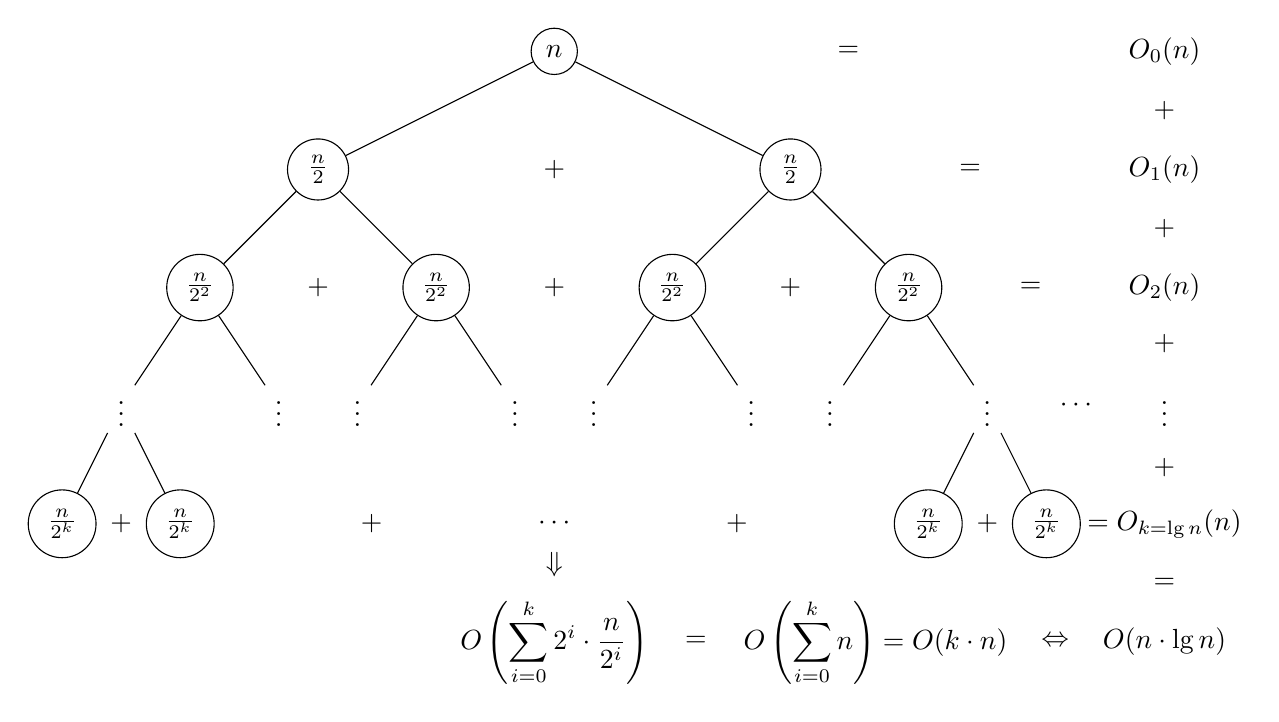
\begin{tikzpicture}[level/.style={sibling distance=60mm/#1}]
\node [circle,draw] (z){$n$}
  child {node [circle,draw] (a) {$\frac{n}{2}$}
    child {node [circle,draw] (b) {$\frac{n}{2^2}$}
      child {node {$\vdots$}
        child {node [circle,draw] (d) {$\frac{n}{2^k}$}}
        child {node [circle,draw] (e) {$\frac{n}{2^k}$}}
      } 
      child {node {$\vdots$}}
    }
    child {node [circle,draw] (g) {$\frac{n}{2^2}$}
      child {node {$\vdots$}}
      child {node {$\vdots$}}
    }
  }
  child {node [circle,draw] (j) {$\frac{n}{2}$}
    child {node [circle,draw] (k) {$\frac{n}{2^2}$}
      child {node {$\vdots$}}
      child {node {$\vdots$}}
    }
  child {node [circle,draw] (l) {$\frac{n}{2^2}$}
    child {node {$\vdots$}}
    child {node (c){$\vdots$}
      child {node [circle,draw] (o) {$\frac{n}{2^k}$}}
      child {node [circle,draw] (p) {$\frac{n}{2^k}$}
          child [grow=right] {node (q) {$ = O_{k = \lg n}(n)$} edge from parent[draw=none]
            child [grow=up] {node (r) {$\vdots$} edge from parent[draw=none]
              child [grow=up] {node (s) {$O_2(n)$} edge from parent[draw=none]
                child [grow=up] {node (t) {$O_1(n)$} edge from parent[draw=none]
                  child [grow=up] {node (u) {$O_0(n)$} edge from parent[draw=none]}
                }
              }
            }
            child [grow=down] {node (v) {$O(n \cdot \lg n)$}edge from parent[draw=none]}
        }
      }
    }
  }
};
\path (a) -- (j) node [midway] {+};
\path (b) -- (g) node [midway] {+};
\path (k) -- (l) node [midway] {+};
\path (k) -- (g) node [midway] {+};
\path (d) -- (e) node [midway] {+};
\path (o) -- (p) node [midway] {+};
\path (o) -- (e) node (x) [midway] {$\cdots$}
  child [grow=down] {
    node (y) {$O\left(\displaystyle\sum_{i = 0}^k 2^i \cdot \frac{n}{2^i}\right)$}
    edge from parent[draw=none]
  };
\path (q) -- (r) node [midway] {+};
\path (s) -- (r) node [midway] {+};
\path (s) -- (t) node [midway] {+};
\path (s) -- (l) node [midway] {=};
\path (t) -- (u) node [midway] {+};
\path (z) -- (u) node [midway] {=};
\path (j) -- (t) node [midway] {=};
\path (y) -- (x) node [midway] {$\Downarrow$};
\path (v) -- (y)
  node (w) [midway] {$O\left(\displaystyle\sum_{i = 0}^k n\right) = O(k \cdot n)$};
\path (q) -- (v) node [midway] {=};
\path (e) -- (x) node [midway] {+};
\path (o) -- (x) node [midway] {+};
\path (y) -- (w) node [midway] {$=$};
\path (v) -- (w) node [midway] {$\Leftrightarrow$};
\path (r) -- (c) node [midway] {$\cdots$};
\end{tikzpicture}}
\caption{Lorem ipsum dolor sit amet}\label{img:index}
\end{figure}

%---------------------------------------------------------------
\section{Ut enim ad minim veniam}
%---------------------------------------------------------------

\lipsum[2-4]

%---------------------------------------------------------------
\subsection{Ut enim ad minim veniam}
%---------------------------------------------------------------

Curabitur ligula sapien, pulvinar a vestibulum quis, facilisis vel sapien. Duis condimentum augue id magna semper rutrum. Aliquam ornare wisi eu metus. Fusce aliquam vestibulum ipsum. Vivamus ac leo pretium faucibus~\ref{img:index}.

\begin{itemize}
    \item Ut enim ad minim veniam, quis nostrud
    \item Ut enim ad minim 
    \item Ut enim ad minim veniam, quis 
    \begin{itemize}
        \item Ut enim ad
        \item Ut enim ad
        \begin{itemize}
            \item Ut enim 
            \item Ut enim 
            \begin{itemize}
            \item Ut enim 
            \item Ut enim 
        \end{itemize}
        \end{itemize}
    \end{itemize}
\end{itemize}

\section{Class aptent taciti}


Even though dark mode can be very nice for websites and apps, it does not look good when printed. Consider using white mode when print-screening dark-moded content. The contrast with the white page is too big, as seen in Figure~\ref{fig:Darkmode}.

\begin{figure}[!htbp]
    \centering
    \includegraphics[width=\linewidth]{images/darkmode}
    \caption{White and dark mode comparison.~\cite{darkMode}}
    \label{fig:Darkmode}
\end{figure}


\subsection{Class aptent taciti}

\lipsum[6-7]

\begin{enumerate}
    \item Ut enim ad minim veniam, quis nostrud
    \item Ut enim ad minim 
    \item Ut enim ad minim veniam, quis 
    \begin{enumerate}
        \item Ut enim ad
        \item Ut enim ad
        \begin{enumerate}
            \item Ut enim 
            \item Ut enim 
            \begin{enumerate}
            \item Ut enim 
            \item Ut enim 
        \end{enumerate}
        \end{enumerate}
    \end{enumerate}
\end{enumerate}


%---------------------------------------------------------------
\section{Ut enim ad minim veniam, quis nostrud}
%---------------------------------------------------------------

Ut enim ad minim veniam, quis nostrud exercitation ullamco laboris nisi ut aliquip ex ea commodo consequat. Nulla non arcu lacinia neque faucibus fringilla. Vestibulum erat nulla, ullamcorper nec, rutrum non, nonummy ac, erat. Aliquam erat volutpat. Proin pede metus, vulputate nec, fermentum fringilla, vehicula vitae, justo.\footnote{Ut enim ad minim veniam, quis nostrud exercitation.} Etiam dictum tincidunt diam. In laoreet, magna id viverra tincidunt, sem odio bibendum justo, vel imperdiet sapien wisi sed libero. Nulla est. Maecenas fermentum, sem in pharetra pellentesque, velit turpis volutpat ante, in pharetra metus odio a lectus. Duis aute irure dolor in reprehenderit in voluptate velit esse cillum dolore eu fugiat nulla pariatur. 

\begin{lstlisting}[caption={Zbytečný kód},label=list:8-6,captionpos=b,float,abovecaptionskip=-\medskipamount,abovecaptionskip=\medskipamount,language=C]
    #include<stdio.h>
    #include<iostream>
    // A comment
    int main(void)
    {
        printf("Hello World\n");
        return 0;
    }
\end{lstlisting}

%%%%%%%%%%%%%%%%%%%%%%%%%%%%%%%%%
% alternative using package minted for source highlighting
% package minted requires execution with `-shell-escape'
% e.g., `xelatex -shell-escape ctufit-thesis.tex'
% \begin{listing}
% \begin{minted}{C}
%     #include<stdio.h>
%     #include<iostream>
%     // A comment
%     int main(void)
%     {
%         printf("Hello World\n");
%         return 0;
%     }
% \end{minted}
% \caption{Zbytečný kód}\label{list:8-6}
% \end{listing}
% %%%%%%%%%%%%%%%%%%%%%%%%%%%%%%%%%
Nullam feugiat, turpis at pulvinar vulputate, erat libero tristique tellus, nec bibendum odio risus sit amet ante. Aenean id metus id velit ullamcorper pulvinar. Fusce wisi. Integer lacinia. Aliquam id dolor. Pellentesque pretium lectus id turpis. Suspendisse sagittis ultrices augue. In laoreet, magna id viverra tincidunt, sem odio bibendum justo, vel imperdiet sapien wisi sed libero. Sed ac dolor sit amet purus malesuada congue.~\cite{Crochemore2002}

Class aptent taciti sociosqu ad litora torquent per conubia nostra, per inceptos hymenaeos. Fusce suscipit libero eget elit. Etiam dui sem, fermentum vitae, sagittis id, malesuada in, quam. Aliquam id dolor. Curabitur bibendum justo non orci. Duis viverra diam non justo. Curabitur ligula sapien, pulvinar a vestibulum quis, facilisis vel sapien. Duis condimentum augue id magna semper rutrum. Aliquam ornare wisi eu metus. Fusce aliquam vestibulum ipsum. Vivamus ac leo pretium faucibus.~\cite{Motwani2014}

%---------------------------------------------------------------
\subsection{Ut enim ad minim veniam, quis nostrud}
%---------------------------------------------------------------

Ut enim ad minim veniam, quis nostrud exercitation ullamco laboris nisi ut aliquip ex ea commodo consequat. Nulla non arcu lacinia neque faucibus fringilla. Vestibulum erat nulla, ullamcorper nec, rutrum non, nonummy ac, erat. Aliquam erat volutpat. Proin pede metus, vulputate nec, fermentum fringilla, vehicula vitae, justo. Etiam dictum tincidunt diam. In laoreet, magna id viverra tincidunt, sem odio bibendum justo.~\cite{Sestakova2018} 

% \begin{table}\centering
% \begin{tabular}{l|l|c|c}
% 	Typ		& Prostředí		& \LaTeX{}ovská zkratka	& \TeX{}ovská zkratka	\tabularnewline \hline 
%  	Text		& \verb|math|		& \verb|\(...\)|	& \verb|$...$|	\tabularnewline \hline
%  	Displayed	& \verb|displaymath|	& \verb|\[...\]|	& \verb|$$...$$|	\tabularnewline 
% \end{tabular}
% \caption[Příklad tabulky]{Zadávání matematiky}
% \label{tab:matematika}
% \end{table}


Nulla est. Maecenas fermentum, sem in pharetra pellentesque, velit turpis volutpat ante, in pharetra metus odio a lectus. Duis aute irure dolor in reprehenderit in voluptate velit esse cillum dolore eu fugiat nulla pariatur. Nullam feugiat, turpis at pulvinar vulputate, erat libero tristique tellus, nec bibendum odio risus sit amet ante. Aenean id metus id velit ullamcorper pulvinar. 

\subsubsection{Class aptent taciti}

\begin{definition}[Optional label]
Class aptent taciti sociosqu ad litora torquent per conubia nostra, per inceptos hymenaeos. Fusce suscipit libero eget elit. Etiam dui sem, fermentum vitae, sagittis id, malesuada in, quam. Aliquam id dolor. Curabitur bibendum justo non orci.
\end{definition}

\begin{example}
Class aptent taciti sociosqu ad litora torquent per conubia nostra, per inceptos hymenaeos. Fusce suscipit libero eget elit. Etiam dui sem, fermentum vitae, sagittis id, malesuada in, quam. Aliquam id dolor. Curabitur bibendum justo non orci.
\end{example}

\paragraph{Nadpis 5. úrovně}

\begin{theorem}
Class aptent taciti sociosqu ad litora torquent per conubia nostra, per inceptos hymenaeos. Fusce suscipit libero eget elit. Etiam dui sem, fermentum vitae, sagittis id, malesuada in, quam. Aliquam id dolor. Curabitur bibendum justo non orci.
\end{theorem}

\begin{proof}
Fusce suscipit libero eget elit. Etiam dui sem, fermentum vitae, sagittis id, malesuada in, quam. Aliquam id dolor. Curabitur bibendum justo non orci.
\end{proof}

\paragraph{Level 5 heading}

\begin{corollary}
Fusce suscipit libero eget elit. Etiam dui sem, fermentum vitae, sagittis id, malesuada in, quam. Aliquam id dolor. Curabitur bibendum justo non orci.
\end{corollary}

\begin{proposition}
Fusce suscipit libero eget elit. Etiam dui sem, fermentum vitae, sagittis id, malesuada in, quam. Aliquam id dolor. Curabitur bibendum justo non orci.
\end{proposition}

\begin{note}
Fusce suscipit libero eget elit. Etiam dui sem, fermentum vitae, sagittis id, malesuada in, quam. Aliquam id dolor. Curabitur bibendum justo non orci.
\end{note}

\begin{remark}
Fusce suscipit libero eget elit. Etiam dui sem, fermentum vitae, sagittis id, malesuada in, quam. Aliquam id dolor. Curabitur bibendum justo non orci.
\end{remark}

\begin{lemma}
Class aptent taciti sociosqu ad litora torquent per conubia nostra, per inceptos hymenaeos. Fusce suscipit libero eget elit. Etiam dui sem, fermentum vitae, sagittis id, malesuada in, quam. Aliquam id dolor. Curabitur bibendum justo non orci.
\end{lemma}

\lipsum[1-2]

% \subsection{Class aptent taciti sociosqu}
% 
% \lipsum[4-5]

%---------------------------------------------------------------
\chapter{Lorem ipsum}
%---------------------------------------------------------------

\begin{chapterabstract}
	Lorem ipsum dolor sit amet, consectetuer adipiscing elit. Curabitur sagittis hendrerit ante. Class aptent taciti sociosqu ad litora torquent per conubia nostra, per inceptos hymenaeos. Cras pede libero, dapibus nec, pretium sit amet, tempor quis. Sed vel lectus. Donec odio tempus molestie, porttitor ut, iaculis quis, sem. Cras pede libero, dapibus nec, pretium sit amet, tempor quis. Sed vel lectus. 
\end{chapterabstract}

Lorem ipsum dolor sit amet, consectetuer adipiscing elit. Curabitur sagittis hendrerit ante. Class aptent taciti sociosqu ad litora torquent per conubia nostra, per inceptos hymenaeos. Cras pede libero, dapibus nec, pretium sit amet, tempor quis. Sed vel lectus. Donec odio tempus molestie, porttitor ut, iaculis quis, sem. Suspendisse sagittis ultrices augue. Donec ipsum massa, ullamcorper in, auctor et, scelerisque sed, est. In sem justo, commodo ut, suscipit at, pharetra vitae, orci. Pellentesque pretium lectus id turpis.~\cite{Kopka2004}

\section{Donec odio tempus molestie}

\lipsum[2]~\cite{def:1, def:2}

\subsection{Class aptent taciti}

\lipsum[2-3]

\begin{description}
\item[Kapitola 1] Lorem ipsum dolor sit amet, consectetuer adipiscing elit. Curabitur sagittis hendrerit ante. Class aptent taciti sociosqu ad litora tor\-quent per conubia nostra, per inceptos hymenaeos. Cras pede libero, dapibus nec, pretium sit amet, tempor quis.

\item[Kapitola 2] Lorem ipsum dolor sit amet, consectetuer adipiscing elit. Curabitur sagittis hendrerit ante. Class aptent taciti sociosqu ad litora tor\-quent per conubia nostra, per inceptos hymenaeos. Cras pede libero, dapibus nec, pretium sit amet, tempor quis.

\item[Kapitola 3] Lorem ipsum dolor sit amet, consectetuer adipiscing elit. Curabitur sagittis hendrerit ante. Class aptent taciti sociosqu ad litora tor\-quent per conubia nostra, per inceptos hymenaeos. Cras pede libero, dapibus nec, pretium sit amet, tempor quis.

\item[Kapitola 4] Lorem ipsum dolor sit amet, consectetuer adipiscing elit. Curabitur sagittis hendrerit ante. Class aptent taciti sociosqu ad litora tor\-quent per conubia nostra, per inceptos hymenaeos. Cras pede libero, dapibus nec, pretium sit amet, tempor quis.~\cite{jakZiskatAcko}
\end{description}

\lipsum[2]

\section{Lorem ipsum dolor sit amet}

\lipsum[3-5]
